% Created 2022-07-11 seg 15:09
% Intended LaTeX compiler: pdflatex
\documentclass[11pt]{article}
\usepackage[utf8]{inputenc}
\usepackage[T1]{fontenc}
\usepackage{graphicx}
\usepackage{longtable}
\usepackage{wrapfig}
\usepackage{rotating}
\usepackage[normalem]{ulem}
\usepackage{amsmath}
\usepackage{amssymb}
\usepackage{capt-of}
\usepackage{hyperref}
\author{Diogo}
\date{\today}
\title{}
\hypersetup{
 pdfauthor={Diogo},
 pdftitle={},
 pdfkeywords={},
 pdfsubject={},
 pdfcreator={Emacs 28.1 (Org mode 9.6)}, 
 pdflang={English}}
\begin{document}

\tableofcontents

\section{Introdução}
\label{sec:org5cf5c8b}
Caro aluno, nesta aula, estudaremos um conjunto de classes e interfaces que compõem o framework Collections da API (Application Programming Interface – Interface de Programação de Aplicação) Java. Esse framework é também chamado de coleções, traduzido para o português, e consiste na implementação das mais importantes estruturas de dados. Aprendendo como funcionam as principais coleções, você estará apto a utilizá-las na construção dos seus programas, economizando tempo de desenvolvimento e garantindo a qualidade de implementação de funcionalidades críticas, como armazenamento e ordenação de dados. Vamos, então, conhecer as coleções?

\textbf{Objetivos}
\begin{itemize}
\item Revisar conceitos sobre as estruturas de dados;
\item Compreender a importância das coleções e a sua implementação;
\item Entender o recurso Generics da linguagem Java.
\end{itemize}

\section{Tópico 1 – Revisão de estrutura de dados e introdução a Coleções}
\label{sec:orgcb00943}
\textbf{Objetivos}
\begin{itemize}
\item Revisar algumas das principais estruturas de dados;
\item Compreender a necessidade do reuso de código de estruturas de dados;
\item Conhecer os componentes base do framework coleções.
\end{itemize}

Como já aprendemos, estruturas de dados são implementações de modelos que têm como objetivo organizar os dados para obter vantagens na manipulação deles. Essas vantagens podem ocorrer em forma de facilidade de manuseio ou de ganho de desempenho.

Vamos revisitar três estruturas de dados normalmente utilizadas em aplicações: a lista, a pilha e a fila. Todas essas estruturas são modelos baseados em conceitos físicos reais de organização de elementos de um mesmo tipo. Neste tópico, faremos uma revisão conceitual de algumas estruturas de dados clássicas que são a base para as coleções. Iniciaremos pela estrutura de dados lista.

\subsection{1.1 Lista}
\label{sec:orged82547}
Uma lista é uma estrutura de dados que se propõe a colocar dados em uma sequência lógica, seja ela a sequência em que os elementos chegaram à lista, a sequência de ordenação baseada nos valores dos elementos ou ainda a sequência que o desenvolvedor quiser.

Uma lista oferece facilidades implícitas para manipulação dos dados que não existem nos vetores, que são estruturas de dados mais simples. Temos como facilidades a adição de elementos em uma determinada posição com o afastamento dos elementos já existentes, alocação dinâmica de memória para adição de elementos além da capacidade inicial da lista etc. A representação gráfica de uma lista é a mesma de um vetor.

Observe, na figura a seguir, um exemplo de uma lista de números de ponto flutuante que representa as notas de um grupo de alunos:

\href{figura1.png}{Figura 1: Exemplo de uma lista de notas de alunos.}

\begin{itemize}
\item Não existem restrições de acesso na lista. Isso quer dizer que é possível ler, adicionar e remover elementos de qualquer posição válida da lista, ou seja, uma posição que esteja dentro dos limites de capacidade dela. A posição 3 é válida para a lista do exemplo dado, enquanto a posição 15 é inválida, pois a última posição da lista, notas\textsubscript{alunos}, é 7.
\end{itemize}

\subsection{1.2 Pilha}
\label{sec:org1b3e6e5}
Uma pilha é uma estrutura de dados similar a uma lista. Ela impõe uma condição de inserção de novos elementos e acesso aos elementos contidos nela. Assim, todo acesso à pilha deve ser feito pelo seu topo, ou seja, existe apenas um local por onde os elementos podem entrar e sair da pilha. Como consequência dessa restrição, uma pilha gera um modelo de manipulação de dados que chamamos de First In, Last Out (FILO), que significa que o primeiro elemento a entrar será o último a sair. Isso ocorre porque, durante o preenchimento da pilha, os novos elementos ficam por cima dos antigos. Assim, um elemento que entrou cedo na pilha só pode sair quando os que vieram depois dele saírem também.

A representação de uma pilha também é semelhante à da lista, porém a pilha, normalmente, é utilizada na orientação vertical. Para ajudar a fixar o conceito de que uns elementos ficam sobre os outros e para ter uma melhor noção do topo da pilha, observe a representação a seguir:

\href{figura2.png}{Figura 2: Representação de uma pilha.}

Um exemplo de utilização da característica de “primeiro a entrar, último a sair” da pilha é a inversão de uma sequência de elementos. Imaginemos uma pilha chamada letras que recebe as letras da palavra “Java”, uma a uma, da esquerda para a direita. Se, em seguida, desempilharmos cada letra, ou seja, removermos cada letra da pilha, e as reunirmos na sequência em que saíram da pilha, formaremos a palavra “avaJ”, que é “Java” ao contrário. Observe, na figura a seguir, as etapas que acabamos de descrever.

\href{figura3.png}{Figura 3: Exemplo de funcionamento de uma pilha.}

\subsection{1.3 Fila}
\label{sec:orgb6c2567}
A fila é uma estrutura de dados que visa representar o modelo de filas convencionais que conhecemos. Certamente, você já deve ter notado que há filas por toda parte. Elas existem em atendimento de supermercados, bancos, quando vamos entrar no ônibus, no avião etc. Diferente da pilha, a fila exige que os novos elementos fiquem no fim da sequência de elementos antigos (existentes) e que a saída de elementos dela ocorra no início da sequência. Chamamos esse comportamento de First In, First Out (FIFO) ou “o primeiro que entra é o primeiro que sai”.

\begin{itemize}
\item Como estrutura de dados, as filas ajudam no tratamento de dados que devem ser sequenciados entre si para que sejam tratados na ordem em que chegaram, inclusive com a possibilidade de alteração. Essa ordem é baseada em prioridades, seguindo a sequência – como ocorre em filas preferenciais de bancos e supermercados – em que uma pessoa que possui prioridade, devido a algum dos seus atributos (idade, deficiência, gravidez etc.), pode ser atendida antes das demais.
\end{itemize}

A seguir, temos uma representação gráfica de uma fila e seu funcionamento. Observe que existem ponteiros que indicam o início e o fim da fila. Esses ponteiros ajudam a identificar onde um novo elemento deve entrar e qual será o próximo a sair.

\href{figura4.png}{Figura 4: Exemplo do funcionamento de uma fila.}

\subsection{1.4 Reuso em estruturas de dados}
\label{sec:org7b74eed}
Agora que relembramos as principais estruturas de dados, vamos pensar em termos de implementação. Escrever classes que representam as estruturas de dados que estudamos até aqui não é uma tarefa das mais complexas mas também não é trivial. Existem diversos fatores que podem tornar complicada a construção de uma estrutura de dados, como segurança, estabilidade, robustez etc.

Nota-se que é relativamente fácil escrever o código de uma estrutura de dados, como uma fila ou uma pilha, mas é necessário muito trabalho e atenção para escrever uma estrutura de dados que seja reutilizável. Por isso, a API Java fornece o framework conhecido como coleções, que contém classes e interfaces voltadas à estruturação e à manipulação de dados, baseado em algoritmos e modelos clássicos da computação.

\begin{itemize}
\item API, como definido em aulas anteriores, é a Interface de Programação de Aplicativos, um conjunto de classes voltado para o desenvolvimento de novas aplicações a partir delas de forma genérica, diferentemente dos frameworks, que têm um foco bem definido. Uma API pode conter um framework.
\end{itemize}

A vantagem de utilizar coleções, em vez de você mesmo implementar as estruturas de dados de que precisa, está no fato de que elas foram criadas e testadas pela equipe de desenvolvimento da linguagem Java e não geram dificuldade de importação, ou seja, estão sempre disponíveis por estarem dentro da API Java. Elas também permitem que apliquemos mais do nosso tempo no desenvolvimento de outras partes do sistema (reuso de software).

\subsection{1.5 Introdução a coleções}
\label{sec:orgbb2b2aa}
Até aqui, revisamos algumas das estruturas de dados mais utilizadas no desenvolvimento de programas em geral. Você pôde notar que utilizar coleções, em vez de você mesmo implementar as estruturas de dados, é mais vantajoso por liberar tempo para o desenvolvimento de outros trechos do projeto ou para facilitar a portabilidade, já que as coleções estão disponíveis na API base do Java. Vamos, agora, entrar na parte mais técnica do estudo de coleções, conhecendo as classes e as interfaces que compõem o framework.

O framework coleções consiste em um conjunto de classes e interfaces voltadas ao agrupamento e à manipulação de dados, normalmente do mesmo tipo, que apresenta bom desempenho e que viabiliza a reutilização de código. Ele está presente na API Java desde a versão 1.2.

Praticamente todos os componentes do framework estão no pacote java.util, que inclui também outras diversas classes e interfaces voltadas às tarefas cotidianas do desenvolvimento de software, como geração de números aleatórios, entrada e saída de dados, tratamento de Zona de Hora e formatação de String.

As interfaces base desse framework são Collection e Iterable. Iterable possui apenas o método iterator(). Esse método deve fornecer um objeto do tipo Iterable, capaz de percorrer uma coleção de dados de forma iterativa, ou seja, sequencial, através de três métodos:

hasNext() – indica se ainda existe algum elemento na coleção que ainda não foi visitado;
next() – entrega uma referência para o elemento atual;
remove() – remove o elemento atual da coleção que está sendo iterada.

Já a interface Collection possui uma lista de métodos que visam fornecer a capacidade de adição e remoção de elementos na coleção, cálculo da quantidade de elementos presentes nela, busca de elementos, limpeza da coleção (eliminação de todos os elementos de uma só vez) e transformação da coleção em um vetor simples.

Juntas, as interfaces Iterable e Collection (que estende Iterable) fornecem um conjunto de métodos a serem implementados nas classes concretas de coleções que as tornam capazes de representar, de forma mínima, uma coleção de elementos. Existe mais de uma dezena de interfaces que estendem Collection. A partir delas, são criadas as principais classes de coleções que utilizamos no dia a dia.

Chegamos ao fim do tópico 1. Nele, relembramos algumas estruturas de dados abordadas e percebemos a importância de reutilizarmos o código quando trabalhamos com essas estruturas. Conhecemos, também, a base do framework coleções. Agora, estudaremos a implementação dessas estruturas de forma prática através de classes e interfaces presentes no pacote java.util. Vamos lá?

\section{Tópico 2 – A coleção List}
\label{sec:orge8edf71}
\textbf{Objetivos}
\begin{itemize}
\item Conhecer a interface List;
\item Conhecer a principal implementação de List: a classe ArrayList.
\end{itemize}

Estudaremos, agora, o nosso primeiro componente do framework coleções: a interface List. Essa interface visa representar uma lista. Conforme abordado no tópico anterior, uma lista é uma estrutura de dados que oferece uma série de funcionalidades extras de inserção, remoção e manipulação dos dados que armazena.

Os elementos de uma lista formam uma sequência ordenada, portanto, a ordem com que são inseridos na lista é importante. Para isso, são oferecidos dois métodos de inserção de elementos:

mOs elementos de uma lista formam uma sequência ordenada, portanto, a ordem com que são inseridos na lista é importante. Para isso, são oferecidos dois métodos de inserção de elementos:

método add(Object elemento): adiciona o objeto elemento no fim da lista;
método add(int indice, Object elemento): adiciona o objeto elemento na posição indicada da lista. Se houver elementos na posição indicada ou depois dela todos eles serão movidos para que o novo elemento seja colocado exatamente onde foi requisitado.

Além dos métodos voltados à inserção de elementos, existem métodos especiais para a alteração de um elemento existente, obtenção do índice de um determinado elemento dentro da lista, acesso a um elemento da lista sem removê-lo (essa funcionalidade não existe na interface Collection, que dá acesso ao elemento apenas se ele for removido da lista) e criação de sublistas, ou seja, de trechos da lista original.

Assim como os vetores, as listas têm suas posições baseadas em 0 (zero), ou seja, o índice do seu primeiro elemento é 0 (zero). É importante mencionar que listas são coleções que permitem a existência de elementos duplicados. Você conhecerá, mais adiante, outros tipos de coleção que previnem a inserção de elementos nulos ou repetidos.

Lembre-se de que List é uma interface, não uma classe. Logo, você não pode instanciar um objeto diretamente de List. Para isso, precisamos de uma classe concreta que implemente a List. Diversas classes implementam essa interface, como ArrayList, AttributeList, Stack, Vector e LinkedList. Agora, vamos nos aprofundar no estudo da classe ArrayList.étodo add(Object elemento): adiciona o objeto elemento no fim da lista;
método add(int indice, Object elemento): adiciona o objeto elemento na posição indicada da lista. Se houver elementos na posição indicada ou depois dela todos eles serão movidos para que o novo elemento seja colocado exatamente onde foi requisitado.

Além dos métodos voltados à inserção de elementos, existem métodos especiais para a alteração de um elemento existente, obtenção do índice de um determinado elemento dentro da lista, acesso a um elemento da lista sem removê-lo (essa funcionalidade não existe na interface Collection, que dá acesso ao elemento apenas se ele for removido da lista) e criação de sublistas, ou seja, de trechos da lista original.

Assim como os vetores, as listas têm suas posições baseadas em 0 (zero), ou seja, o índice do seu primeiro elemento é 0 (zero). É importante mencionar que listas são coleções que permitem a existência de elementos duplicados. Você conhecerá, mais adiante, outros tipos de coleção que previnem a inserção de elementos nulos ou repetidos.

Lembre-se de que List é uma interface, não uma classe. Logo, você não pode instanciar um objeto diretamente de List. Para isso, precisamos de uma classe concreta que implemente a List. Diversas classes implementam essa interface, como ArrayList, AttributeList, Stack, Vector e LinkedList. Agora, vamos nos aprofundar no estudo da classe ArrayList.

\subsection{2.1 A classe ArrayList}
\label{sec:orgf1e13b7}
A implementação concreta mais utilizada de List é ArrayList, principalmente pela sua simplicidade, o que a torna uma boa opção para a maioria dos casos. Basicamente, ArrayList disponibiliza todas as operações descritas em List e a opção extra de informar a capacidade inicial da lista. É possível descartar posições vazias da lista durante sua utilização, liberando memória que não está sendo utilizada. Como se trata de uma implementação direta de List, um ArrayList permite a inclusão de elementos nulos.

Observe, a seguir, um trecho de código que utiliza um ArrayList para armazenar uma lista de objetos do tipo String.

\begin{verbatim}
    /* Instanciando o objeto 'lista' */
        ArrayList lista = new ArrayList(50);

        /* Adicionando elementos à lista */
        lista.add("João");
        lista.add("Gisele");
        lista.add("Pedro");
        lista.add(1,"Ana");

        /* Exibindo o índice do elemento "Ana" */
        System.out.println("Ana está na posição: " + lista.indexOf("Ana"));

        /* Apagando todos os elementos da lista */
        lista.clear();

        /* Exibindo o tamanho da lista após usar clear() */
        System.out.println("Tamanho atual da lista: " + lista.size());
\end{verbatim}

No exemplo, declaramos um objeto chamado lista do tipo ArrayList e utilizamos o construtor de ArrayList que recebe um parâmetro inteiro, que será usado para definir o tamanho inicial da lista. Foi passado o valor 50, mas, se não tivéssemos fornecido um valor, a lista seria criada com capacidade inicial de 10 itens. Isso significa que a lista foi criada em memória, mas tem capacidade de 50, no entanto, pode ser aumentada automaticamente à medida que novos itens sejam inseridos. Não confunda capacidade com tamanho. Capacidade é a quantidade de itens que a lista suporta em determinado momento. Tamanho é a quantidade de itens que ela está armazenando no determinado momento.

Em seguida, utilizamos duas assinaturas do método add(): uma que recebe apenas um parâmetro, com o qual adicionamos 3 (três) elementos (João, Gisele e Pedro), sempre no fim da lista; e a outra que recebe um parâmetro inteiro extra além do elemento a ser inserido. Neste último, o parâmetro indica em que posição da lista o elemento deve ser alocado. Nesse caso, a lista que tinha João na posição 0 (zero), Gisele na posição 1 (um) e Pedro na posição 2 (dois), após a execução de lista.add(1, “Ana”), passou a ter a seguinte configuração: João na posição 0 (zero), Ana na posição 1 (um), Gisele na posição 2 (dois) e Pedro na posição 3 (três). Perceba que todos os elementos da posição 1 (um) em diante foram movidos.

Após isso, usamos o método indexOf() para identificar em que posição está o elemento “Ana”. Caso o elemento não seja encontrado, esse método retorna o valor -1. Utilizamos também o método clear() para excluir todos os elementos presentes na lista. Por fim, o método size() foi usado para informar o tamanho da lista que, após o uso de clear(), deve ser igual a 0 (zero).

Chegamos ao fim do tópico 2. Estudamos uma das coleções mais simples, a List, que corresponde a um conjunto de elementos ordenados e sem restrições de acesso. Estudamos um exemplo de implementação dessa coleção com a classe ArrayList e alguns métodos úteis, específicos dessa classe, que facilitam bastante a manipulação dos dados armazenados na coleção. A seguir, estudaremos a coleção Stack.

\section{Tópico 3 – A coleção Stack}
\label{sec:org0e90a3f}
\textbf{Objetivo}
\begin{itemize}
\item Conhecer a classe Stack.
\end{itemize}

No estudo de estrutura de dados, conceituamos Pilha. No framework coleções, a classe Stack representa uma pilha com todos os comportamentos previstos pelo modelo. A nomenclatura dos métodos também segue o padrão de push para adição de elementos e pop para remoção.

A classe Stack é subclasse de Vector, uma implementação de List que possui algumas particularidades voltadas à gerência de aumento e diminuição dinâmica do tamanho da coleção. Por exemplo, um construtor da classe Vector possui um atributo chamado capacityIncrement que define a quantidade de posições que a coleção deve aumentar quando o limite da capacidade for alcançado em uma operação de adição de elementos. Vector e Stack permitem a existência de elementos nulos.

Observe, a seguir, um exemplo de uso da classe Stack:

\begin{verbatim}
    /* Instanciação da Pilha */
        Stack pilha = new Stack();

        /* Texto a ser empilhado */
        String texto = "ABCDE";
        /* Empilhando letra a letra */
        for(char c : texto.toCharArray()){
            pilha.push(c);
        }
        /* Vendo o elemento no topo da pilha */
        System.out.println("Elementos no topo da pilha: " + pilha.peek());

        /* Exibindo a quantidade de elementos na pilha */
        System.out.println("Quantidade de elementos na pilha: " + pilha.size());

        /* Desempilhando */
        String textoInvertido = "";
        while(!pilha.isEmpty()){
            textoInvertido += pilha.pop();
        }

        /* Exibindo o texto formado no desempilhamento */
        System.out.println("Texto obtido na inversão: " + textoInvertido);
\end{verbatim}

O exemplo ilustra o que foi proposto no tópico 1, quando mencionamos sobre Pilhas, invertendo a palavra “Java”, usando empilhamento e desempilhamento. Empilhamos as letras do texto “ABCDE” e, em seguida, removemos todas elas, formando “EDCBA”.

O for-each é uma variação do laço for tradicional. A sua estrutura é simples: for (variável auxiliar: coleção) \{ corpo do laço \}. Primeiro, declaramos uma variável auxiliar do tipo de objeto ou dado que a coleção armazena; depois, declaramos a coleção a qual desejamos iterar. A ideia é simples: para cada elemento da coleção, a variável auxiliar assume a referência do objeto ou valor de dado disponível. Isso se repete até não restar elementos da coleção para se visitar.

O construtor de Stack é o único que não recebe parâmetros, criando uma instância de coleção vazia. Através do método push, adicionamos cada uma das letras do texto “ABCDE” à pilha. Ao fim do laço, a pilha deve estar como exibido na próxima figura:

\begin{center}
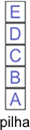
\includegraphics[width=.9\linewidth]{figura5.png}
\end{center}
Figura 5: Estado da pilha após adição das letras.

Utilizamos o método peek() para conferir o elemento que está no topo da pilha. Assim como fizemos com ArrayList, podemos utilizar o método size() (que vem da interface List) para saber quantos elementos existem na pilha no momento. Por fim, utilizamos o método pop() para remover os elementos da pilha, sempre a partir do topo, e o método isEmpty() (que também é descendente da interface List) para verificar se a coleção está vazia.

De forma geral, o uso de Stack ocorre apenas quando precisamos manter os elementos em uma sequência muito específica sendo, geralmente, a sequência inversa de aquisição dos dados ou quando se precisa trabalhar com duas ou mais fontes de dados. Um bom exemplo do uso de pilhas é o processo de tratamento de expressões matemáticas em uma calculadora.

Quando você digita a expressão 5 * (3 + 8) na calculadora, ela usa duas pilhas para armazenar cada tipo de elemento da expressão: uma pilha para operadores e uma para números. Assim, lendo a expressão da esquerda para a direita e colocando cada elemento na sua pilha correta, as duas pilhas ficam da seguinte forma:

\href{figura6.png}{Figura 6: Exemplo de representação de pilhas.}

O processo de resolução da expressão começa pela leitura dos elementos no topo da pilha de operadores. No caso, temos um fechamento de parênteses, que é descartado. Em seguida, temos um operador de soma. Nesse momento, retiramos o número do topo da pilha de números e somamos ao novo topo, ou seja, o que está embaixo dele, no nosso exemplo, 8 e 3. O resultado, 11, é empilhado na pilha de números e o processo continua.

O próximo elemento no topo da pilha de operadores é referente à abertura de parênteses, que é descartado. Em seguida, existe um operador de multiplicação. Então retiramos o elemento no topo da pilha de números, 11, e o multiplicamos pelo novo topo, que é igual a 5, obtendo 55. Empilhamos 55 na pilha de números. Como não restam mais operadores na pilha de operadores, o resultado da expressão foi encontrado, e é igual a 55.

\href{figura7.png}{Figura 7: Exemplo de representação de pilhas.}

Como você pôde perceber, o uso de pilhas é bem mais específico que o uso de listas, o que implica que a utilização da classe Stack é menos frequente que o uso de ArrayList, por exemplo. Analise a sua aplicação e avalie se existe a necessidade de implementação de uma pilha ou se apenas uma lista convencional completa as suas necessidades.

Chegamos ao fim do tópico 3. Até este momento, estudamos coleções que são baseadas na interface List, como ArrayList e Stack. A interface List oferece uma série de métodos que nos permite criar coleções com comportamento de lista, ou seja, conjuntos de elementos nos quais a ordem entre eles é importante e que permite repetições. No próximo tópico, estudaremos a coleção Set.

\section{Tópico 4 – A coleção Set}
\label{sec:org71b583c}
\textbf{Objetivo}
\begin{itemize}
\item Conhecer a interface Set e a sua principal implementação: a classe HashSet.
\end{itemize}

A coleção Set tem uma característica diferente das outras coleções apresentadas até agora. Set é uma interface que está no mesmo nível de List, ou seja, herda diretamente de Collection e, portanto, define comportamentos não necessariamente iguais aos de List e suas implementações.

O diferencial da interface Set é que ela é a base para implementação de estruturas que não permitem duplicidade, assim, dentro de um Set, não existem elementos iguais. Isso decorre do fato de Set ser um modelo baseado nos conjuntos da matemática. Em conjuntos, quando se tenta adicionar um elemento “X” que já existe em um conjunto “A”, nada é feito, porque “X” já pertence a “A”.

Observe a figura a seguir para compreender melhor o conceito de controle de duplicidade em conjuntos.

\href{figura8.png}{Figura 8: Adição de elementos a um conjunto fictício Z.}

Vamos acompanhar o que ocorre na figura. No Estado 1, temos o conjunto “Z” vazio. A tentativa de adição de um elemento “a” nos leva ao Estado 2, em que, dentro do conjunto “Z”, podemos observar a presença de “a”. Em seguida, tentamos adicionar novamente um elemento “a”. Como “a” já existe em “Z”, nada é modificado em “Z”, e chegamos ao Estado 3, que é exatamente igual ao Estado 2. Por fim, tentamos adicionar “b” a “Z”, com sucesso, chegando ao Estado 4.

Da mesma forma, em coleções derivadas da interface Set, como o HashSet, não ocorre duplicação, pois, antes de adicionar qualquer elemento à coleção, ocorre um teste para verificar se o elemento é nulo ou se ele já existe. Uma vez validado, o elemento pode entrar na coleção.

Sets não provêm de métodos para ter acesso direto aos seus elementos, sendo que o desenvolvedor deve utilizar o método iterator (descrito no fim do tópico 1) para obter um objeto que faça a iteração sobre todos os elementos dessa coleção. De posse de um objeto do tipo iterator, e usando os métodos hasNext e next, é possível percorrer os elementos do Set e manipulá-los.

\subsection{4.1 A classe HashSet}
\label{sec:org0dfc094}
A principal implementação concreta de Set é o HashSet. Conheceremos um exemplo simples do uso de HashSet e comprovaremos que não é possível colocar dois elementos com o mesmo valor em uma coleção do tipo Set.

\begin{verbatim}
    HashSet hash = new HashSet();
        hash.add("Teste");
        hash.add("Teste");
        hash.add("Teste 2");
        System.out.println("Qtd. de Elementos: " + hash.size());
\end{verbatim}

No exemplo, instanciamos um objeto hash do tipo HashSet e, em seguida, tentamos adicionar duas vezes o elemento “Teste” e uma vez o elemento “Teste 2”. Depois, exibimos uma mensagem com a quantidade de elementos que existe na coleção hash. Se você executar o trecho de código da figura, terá como saída o texto “Qtd. de Elementos: 2”. Isso significa que, em vez de 3 (três) elementos, referentes às 3 (três) inserções que fizemos com o método add(), existem apenas 2 (dois) elementos distintos na coleção, que são “Teste” e “Teste 2”.

Chegamos ao fim do tópico 4. Estudamos a coleção Set e a sua principal implementação, HashSet. Sets são muito úteis quando se deseja garantir que a coleção de elementos não possua duplicidade. Essa característica é bem explorada por frameworks de bancos de dados que recuperam dados, montam objetos de classes que refletem o modelo de tabelas do banco de dados e disponibilizam os objetos em Sets que previnem a duplicidade. Estudaremos alguns usos de Sets durante o nosso curso.

\section{Tópico 5 – A coleção Map}
\label{sec:orgfca613c}
\textbf{Objetivo}
\begin{itemize}
\item Conhecer a interface Map e a sua principal implementação, a classe HashMap.
\end{itemize}

A interface Map permite a criação de coleções conhecidas como mapas ou dicionários que favorecem a busca por seus elementos através da associação entre chaves e valores. Quando inserimos um novo elemento em um mapa, devemos adicionar também uma chave que o identifique para que, através dela, possamos encontrá-lo posteriormente. Essa chave pode ser de tipo primitivo, como inteiros, números de ponto flutuante ou caracteres, ou ainda objetos complexos, como String, JFrame ou outro objeto criado a partir de classes próprias.

\begin{itemize}
\item Embora a palavra mapa nos remeta à ideia de mapa geográfico, o conceito que é adotado na aula é apenas o de que um mapa relaciona um local a um nome ou coordenada que o identifique.
\item Em programação, ele é uma espécie de tabela que relaciona um identificador a um valor. Por isso, também é conhecido como dicionário. Em termos de código, pode ser implementado usando matrizes, listas, árvores ou outras estruturas de dados.
\end{itemize}

A interface Map provê métodos para inserção, remoção e busca de elementos ou chaves dentro de seu conjunto. Esses métodos podem ser divididos em cinco. Observe:

\textbf{put(chave, elemento)}: recebe um elemento a ser inserido na coleção e na chave a qual o elemento estará associado;
\textbf{get(chave)}: devolve o elemento associado à chave fornecida, se ele existir;
\textbf{remove(chave)}: remove o elemento associado à chave fornecida, se ele existir;
\textbf{keySet()}: devolve um Set de todas as chaves da coleção;
\textbf{values()}: devolve um Collection de todos os elementos contidos na coleção.

Na próxima seção, vamos estudar uma das implementações de Map: a classe HashMap, responsável pela criação de mapas ou dicionários que, embora não garantam um padrão sobre a ordem interna dos elementos, permitem que os acessemos diretamente através de suas chaves. Vamos lá!

\subsection{5.1 A classe HashMap}
\label{sec:orgce15961}
A principal implementação concreta de Map é o HashMap. Ela permite que adicionemos tanto chaves nulas quanto elementos nulos, mas mantém a característica de não permitir elementos ou chaves duplicadas. Outra característica é que um HashMap não garante a ordem dos elementos dentro da coleção, por exemplo, que a ordem seja a mesma de inserção ou que a ordem seja mantida durante o uso. A seguir, é apresentado um exemplo simples de HashMap:

\begin{verbatim}
  /* Criando o mapa */
    HashMap mapa = new HashMap();

    /* Adicionando elementos */
    mapa.put(5, "Cinco");
    mapa.put(2.5f, "Dois e meio");
    mapa.put('c', "Letra C");
    mapa.put(new Object(), new ArrayList());

    /* Buscando um elemento através da chave */
    char chave = 'c';
    System.out.println("O elemento associado à chave " + chave + " é " + mapa.get(chave));

    /* Exibindo todos os elementos da coleção */
    for (Object obj : mapa.values()) {
        System.out.println(obj);
    }
\end{verbatim}

No exemplo anterior, instanciamos um objeto hash do tipo HashMap e, em seguida, adicionamos quatro elementos distintos, sendo três deles do tipo String e um do tipo ArrayList. Já como chaves para esses elementos, utilizamos quatro tipos diferentes: inteiro, número de ponto flutuante, caractere e Object. Observe a representação do estado interno do mapa após a inserção de todos os elementos:

\emph{Quadro 1: Representação dos dados armazenados no mapa.}
\begin{center}
\begin{tabular}{ll}
Chave & Valor\\
\hline
5 & ``Cinco''\\
c & ``Letra c''\\
2.5 & ``Dois e meio''\\
object & ArrayList\\
\end{tabular}
\end{center}

Lembre-se de que não é possível garantir que essa seja a sequência dos pares chave/valor na memória do computador. Ainda no exemplo do código anterior, utilizamos o método get() para encontrar um elemento dentro da coleção, passando uma chave como parâmetro. Caso essa chave não exista na coleção, o retorno do método get() será nulo. Por fim, utilizamos o método values() para obter um Collection de todos os elementos da coleção e, utilizando um laço for, exibimos todos eles no quadro.

Chegamos ao fim do tópico 5. Estudamos os mapas, um tipo de coleção que, assim como os Sets, não permite a repetição de elementos. Os mapas são muito práticos de usar por fornecer uma maneira de acesso direto ao elemento buscado através da chave. Isso nos possibilita a não ter que percorrer toda a lista de elementos em busca do que precisamos.

A seguir, estudaremos um recurso da API Java: Generics.

\section{Tópico 6 – Uso do Generics}
\label{sec:org667234e}
\textbf{Objetivos}
\begin{itemize}
\item Conhecer o recurso Generics;
\item Entender como aplicar Generics associado às coleções.
\end{itemize}

Estudamos que as coleções nos ajudam a organizar nossos dados de forma mais robusta e eficiente, mas você deve ter percebido um inconveniente, sobretudo quando trabalhamos com Hashtables, em que é necessário manipular chaves e valores: a conversão de Object para o tipo de dados que queremos.

Observe o código a seguir. Nele, temos a classe TesteDeGenerics, que contém um objeto do tipo T e um método que exibe os dados desse objeto na tela.

\begin{verbatim}
    public class TesteDeGenerics<T> {
            private T meuObjeto;

            public TesteDeGenerics(T objeto) {
                    meuObjeto = objeto;
            }

            public void exibirInformacaoDoObjeto(){
                System.out.println(meuObjeto.toString());
            }

            public static void main(String[] args) {
                TesteDeGenerics<String> t1 = new TesteDeGenerics<String>("Texto");
                t1.exibirInformacaoDoObjeto();

                TesteDeGenerics<Double> t2 = new TesteDeGenerics<Double>(new Double(99));
                t2.exibirInformacaoDoObjeto();

                TesteDeGenerics<int[]> t3 = new TesteDeGenerics<int[]>(new int[]{10,20,30});
                t3.exibirInformacaoDoObjeto();
            }
        }
\end{verbatim}

Perceba que não definimos nenhum tipo T, ou seja, nenhuma classe chamada T, e que a linguagem Java também não possui uma classe com esse nome. Então, o que significa o T como tipo do objeto meuObjeto na classe do código apresentado? A nomenclatura T é um padrão do recurso Generics e indica ao compilador Java que no lugar de T será inserido o nome real da classe que se pretende usar, mas apenas no momento da instanciação de um objeto da classe TesteDeGenerics ou quando ela for estendida.

O recurso Generics define algumas letras que são reservadas para indicar uma parametrização. Dentre elas, as mais importantes são:

\begin{itemize}
\item E – Elemento;
\item K – Chave (Key);
\item N – Número;
\item T – Tipo;
\item V – Valor.
\end{itemize}

Em especial, utilizaremos as letras E e K, associadas às coleções que estudamos anteriormente, para prevenir a necessidade de conversão manual de objetos do tipo Object para outros tipos. A sintaxe do recurso Generics é simples. Usamos os símbolos “menor que” (<) e “maior que” (>) como delimitadores e, entre eles, indicamos todos os tipos de parâmetros que serão necessários. No exemplo do código citado, tínhamos:


\begin{verbatim}
    public class TesteDeGenerics<T> {
            /* ... */
        }
\end{verbatim}

Perceba o T entre os símbolos “menor que” e “maior que”. Isso indica que a classe TesteDeGenerics precisará da definição de um tipo de referência e toda ocorrência de T, no código-fonte de TesteDeGenerics, deverá ser substituída pelo tipo indicado. É o que ocorre quando instanciamos o objeto t3 no método main da classe TesteDeGenerics, quando passamos vetor de inteiros (int[]) como referência de tipo a ser substituído em todas as ocorrências de T, como pode ser notado no código a seguir. Isso também ocorre para os objetos t1 e t2, mas os tipos passados foram String e Double, respectivamente.

\begin{verbatim}
    public class TesteDeGenerics<T> {
            publicstaticvoid main(String[] args) {
                /* ... */
                TesteDeGenerics<int[]> t3 =
                    new TesteDeGenerics<int[]>(new int[]{10,20,30});
                /* ... */
            }
        }
\end{verbatim}

\subsection{6.1 O uso do Generics em coleções}
\label{sec:orgdac784c}
A aplicação do recurso Generics em coleções é bastante útil para reduzir a codificação de casts manuais para manuseio de elementos oriundos dessas coleções.

\begin{itemize}
\item Antes da criação do recurso Generics, o desenvolvedor era obrigado a converter manualmente todos os elementos (objetos) que vinham de dentro de uma coleção, aumentando a quantidade de código e abrindo brechas para possíveis exceções em tempo de execução do programa.
\end{itemize}

Coleções List e Set demandam apenas o uso da parametrização E de elemento que indicará que todo elemento inserido nela será do tipo E. Nesse caso, o recurso tem uma dupla funcionalidade, pois ele evita que sejam adicionados elementos de tipos diferentes de E e entrega elementos já convertidos para o tipo E (através de método, como get, pop, remove etc.). Observe um exemplo com duas listas que trabalham com e sem o recurso Generics:

Conversão direta com o uso de Generics:

\begin{verbatim}
    ArrayList<Double> listaComGenerics = new ArrayList<Double>();
        listaComGenerics.add(new Double(5));
        Double elemento = listaComGenerics.get(0);
\end{verbatim}

Necessidade de cast quando não se usa Generics:

\begin{verbatim}
    ArrayList listaSemGenerics = new ArrayList();
        listaSemGenerics.add(new Double(5));
        Double elemento = (Double) listaSemGenerics.get(0);
\end{verbatim}

Observe que, no código da conversão direta com o uso de Generics, criamos um ArrayList com a parametrização do tipo de elemento como Double, o que força a verificação de que o elemento que está sendo adicionado à coleção seja do tipo Double. Da mesma forma, quando utilizamos o método get() para recuperar o elemento na posição 0 (zero), obtemos diretamente um objeto do tipo Double, sem necessidade de cast. Já no exemplo seguinte, em que a parametrização de tipo não deve ser feita, na saída do método get(), precisamos aplicar um cast para o tipo Double, porque o método get() devolve apenas objeto do tipo Object.

Para uma única leitura de elemento, pode parecer que não faz grande diferença, mas, se você trabalha com uma coleção de milhares de elementos e em diversos locais no código, a necessidade de fazer cast manualmente é bastante incômoda e improdutiva.

O próximo exemplo do uso de Generics é mais complexo, com parametrização do tipo de chave e elemento em um HashMap.

\begin{verbatim}
    HashMap<String, Double> mapa = new HashMap();
        mapa.put("Elemento 1", new Double(2342.8));
\end{verbatim}

No código, parametrizamos o HashMap mapa de forma que suas chaves ficassem do tipo String e os elementos do tipo Double.

Até aqui, estudamos o framework coleções, que facilita o armazenamento e a busca de elementos em Java. Você pode começar a usar as coleções nos seus programas, substituindo implementações complicadas, utilizando vetores e múltiplas instâncias independentes. Quando você utiliza coleções, sua aplicação ganha em qualidade de código e desempenho, devido ao fato de serem classes e interfaces criadas e testadas a partir de diversos critérios de segurança e qualidade de software pelos mantenedores da linguagem Java.

\begin{itemize}
\item Chegamos ao fim desta aula. Aqui, estudamos a respeito das estruturas de dados e abordamos sobre como criar e manipular arrays, pilhas e filas em Java. Na próxima aula, aprenderemos a documentar nossas classes e gerar um conjunto de arquivos em HTML que contenham documentações sobre o código-fonte, utilizando o aplicativo Javadoc. Até lá!
\end{itemize}
\end{document}
